\chapter{HASIL DAN PEMBAHASAN}
\label{chap:hasildanpembahasan}

% Ubah bagian-bagian berikut dengan isi dari pengujian dan analisis


Pada penelitian ini dipaparkan hasil pengujian berupa implementasi Unreal Engine 5 yang dapat menjalankan sistem dari \emph{Smart Contract Sharing Data}, serta melakukan pengujian terkait
dengan data audio yang diload selama proses sistem berjalan hingga ke tahap pemutaran audio.

\section{Skenario Pengujian}
Pengujian dilakukan dengan melakukan langkah-langkah yang telah ditulis pada bab sebelumnya. Pengujian dimulai dengan melakukan testing method-method yang ada di smart contract.
Fungsi-fungsi yang akan dicoba adalah fungsi yang dibuat sendiri untuk mempermudah proses integrasi. Pengujian dilakukan dengan melibatkan 2 buah akun yang sudah dibuat sebelumnya
menggunakan metamask. Kemudian untuk method-method tersebut juga akan diuji performa dari penggunaan gas dan ETH-nya. Lalu akan dilakukan pengujian integrasi dari Unreal Engine 5.
Pengujian integrasi meliputi berhasil tidaknya melakukan pemutaran audio yang sudah di-\emph{mint} sebelumnya.

\subsection{Hasil Pembuatan Wallet Account}
Pembuatan wallet account dilakukan dengan Metamask. Pada platform metamask dapat dilakukan pembuatan akun dengan menginstall extension browsernya. Setelah terbuat akunnya maka perlu
digunakan faucet untuk mengisi ETH. ETH yang didapat adalah sejumlah 13 GoerliETH. ETH ini sudah lebih dari cukup untuk digunakan. Kemudian dibuat juga akun kedua dan diisikan dengan GoerliETH.
Akun kedua juga dapat digunakan untuk pengujian.


\subsection{Hasil dan Pengujian Method Smart Contract}
Smart Contract yang dibuat dapat digunakan untuk mint NFT. Deployment dilakukan dengan Environment Injected Provider Metamask.
Metamask yang digunakan adalah akun yang sudah dibuat sebelumnya. Contract yang dibuat dideploy sudah digunakan untuk mint NFT.
Untuk pengujian method \texttt{mint}, dilakukan dulu proses deploy dengan menggunakan remix IDE. Contract dideploy di Ganache untuk melakukan pengujian secara lokal karena apabila dilakukan deployment di
Metamask maka ETH yang digunakan akan sulit untuk didapatkan kembali. Berikut ini adalah tabel dari hasil pengujian method \texttt{mint}.
\begin{longtable}{|c|c|}
  \caption{Hasil Pengujian Method \texttt{mint}}
  \label{tb:UjiMint}                              \\
  \hline
  \rowcolor[HTML]{C0C0C0}
  \textbf{URI}              & \textbf{Keterangan} \\
  \hline
  HTTP URL yang berisi JSON & Sukses              \\
  HTTP URL random           & Sukses              \\
  String random             & Sukses              \\
  String kosong             & Gagal               \\
  \hline
\end{longtable}

Pada bagian string kosong akan gagal karena diberikan guard sehingga jika tidak diberikan input maka akan terjadi error.
Sementara untuk string random seperti string yang bukan HTTP URL tidak gagal karena tidak diberikan guard ataupun kondisional yang melakukan
pengecekan terhadap data yang diberikan.

Kemudian untuk bagian method \texttt{getAllTokens} maka akan dilakukan pengujian apakah jumlah id yang dikembalikan sesuai dengan jumlah URI yang sudah di \texttt{mint}.

Kegunaan dari method \texttt{getAllTokens} adalah untuk melakukan query jumlah uri yang ada di blockchain. Maka akan dilakukan pemanggilan \texttt{mint} terlebih dahulu
sebelum melakukan pengujian \texttt{getAllTokens}.

\begin{longtable}{|c|c|}
  \caption{Hasil Pengujian Method \texttt{getAllTokens}}
  \label{tb:UjiGetAllTokens}                                                              \\
  \hline
  \rowcolor[HTML]{C0C0C0}
  \textbf{Jumlah Pemanggilan Mint} & \textbf{Panjang Nilai Balikan \texttt{getAllTokens}} \\
  \hline
  1                                & 1                                                    \\
  2                                & 2                                                    \\
  3                                & 3                                                    \\
  4                                & 4                                                    \\
  5                                & 5                                                    \\
  6                                & 6                                                    \\
  7                                & 7                                                    \\
  8                                & 8                                                    \\
  \hline
\end{longtable}

Dari hasil pengujian dapat dilihat hasilnya adalah sesuai ekspektasi.
Ketika method mint dipanggil sejumlah 1 kali, maka panjang nilai yang dikembalikan oleh method \texttt{getAllTokens} adalah
1. Ketika method mint dipanggil sejumlah 2 kali, maka panjang nilai yang dikembalikan oleh method \texttt{getAllTokens} adalah
2. Ketika method mint dipanggil sejumlah 3 kali, maka panjang nilai yang dikembalikan oleh method \texttt{getAllTokens} adalah
3. Ketika method mint dipanggil sejumlah 4 kali, maka panjang nilai yang dikembalikan oleh method \texttt{getAllTokens} adalah
4. Ketika method mint dipanggil sejumlah 5 kali, maka panjang nilai yang dikembalikan oleh method \texttt{getAllTokens} adalah
5. Ketika method mint dipanggil sejumlah 6 kali, maka panjang nilai yang dikembalikan oleh method \texttt{getAllTokens} adalah
6. Ketika method mint dipanggil sejumlah 7 kali, maka panjang nilai yang dikembalikan oleh method \texttt{getAllTokens} adalah
7. Ketika method mint dipanggil sejumlah 8 kali, maka panjang nilai yang dikembalikan oleh method \texttt{getAllTokens} adalah
8.

Kemudian untuk pengujian method selanjutnya adalah pengujian method \texttt{getAllTokensURI}.
Untuk method ini akan mengembalikan balikan array yang berisi
URI yang sudah disimpan dengan method \texttt{mint} yang sudah pernah dipanggil sebelumnya. Hasil yang diharapkan adalah dengan memanggil method ini maka URI-URI yang sudah pernah
di mint sebelumnya akan dikembalikan dalam bentuk array.

\begin{longtable}{|p{2.5in}|p{2.5in}|}
  \caption{Hasil Pengujian Method \texttt{getAllTokensURI}}
  \label{tb:UjiGetAllTokensURI}                                                                                                                                                                                                                                 \\
  \hline
  \rowcolor[HTML]{C0C0C0}
  \textbf{Mint URI}                                                                                                            & \textbf{Balikan}                                                                                                               \\
  \hline
  https://bafybeu.ipfs.w3s.link/nft-1.json                                                                                     & [https://bafybeu.ipfs.w3s.link/nft-1.json]                                                                                     \\
  https://bafybeu.ipfs.w3s.link/nft-2.json                                                                                     & [https://bafybeu.ipfs.w3s.link/nft-2.json]                                                                                     \\
  https://bafybeu.ipfs.w3s.link/nft-1.json, https://bafybeu.ipfs.w3s.link/nft-2.json                                           & [https://bafybeu.ipfs.w3s.link/nft-1.json, https://bafybeu.ipfs.w3s.link/nft-2.json]                                           \\
  Tidak pernah memanggil method Mint                                                                                           & []                                                                                                                             \\
  https://bafybeu.ipfs.w3s.link/nft-1.json, https://bafybeu.ipfs.w3s.link/nft-2.json, https://bafybeu.ipfs.w3s.link/nft-3.json & [https://bafybeu.ipfs.w3s.link/nft-1.json, https://bafybeu.ipfs.w3s.link/nft-2.json, https://bafybeu.ipfs.w3s.link/nft-3.json] \\
  \hline
\end{longtable}

Dari pemanggilan method-method getAllTokensURI hasilnya adalah sesuai dengan yang diharapkan. Apabila dilakukan mint sebanyak 2 kali maka akan dikembalikan juga sebanyak 2 dan berisikan uri-uri yang sudah pernah di mint sebelumnya.
Apabila dilakukan mint sebanyak 3 kali maka akan dikembalikan juga sebanyak 3 dan berisikan uri-uri yang sudah pernah di mint sebelumnya.
Apabila dilakukan mint sebanyak 4 kali maka akan dikembalikan juga sebanyak 4 dan berisikan uri-uri yang sudah pernah di mint sebelumnya.
Apabila dilakukan mint sebanyak 5 kali maka akan dikembalikan juga sebanyak 5 dan berisikan uri-uri yang sudah pernah di mint sebelumnya.
Method ini akan berguna untuk melakukan pemanggilan di Unreal Engine 5.
Apabila fungsi ini dipanggil oleh Unreal Engine 5 blueprint maka akan dibaca berupa array URI.

Kemudian untuk pengujian method tokenURI akan dilakukan dengan memanggil method mint dan kemudian menggunakan indexnya untuk memanggil  method tokenURI ini. Method ini akan
menggunakan parameter tokenId yang mana adalah urutan dilakukannya mint. Index ini bersifat incremental yang artinya URI pertama memiliki index 0, URI kedua memiliki index 1,
URI ketiga memiliki index 3, URI keempat memiliki index 4, dan URI kelima memiliki index 5, dan seterusnya.

Berikut adalah tabel hasil pengujian method \texttt{tokenURI}

\begin{longtable}{|p{0.5in}|p{2.2in}|p{0.5in}|p{2.2in}|}
  \caption{Hasil Pengujian Method \texttt{tokenURI}}
  \label{tb:UjiTokenURI}                                                                                                                      \\
  \hline
  \rowcolor[HTML]{C0C0C0}
  \textbf{Mint-ke} & \textbf{URI}                             & \textbf{Parameter method tokenURI} & \textbf{Balikan method tokenURI}         \\
  \hline
  1                & https://bafybeu.ipfs.w3s.link/nft-1.json & 0                                  & https://bafybeu.ipfs.w3s.link/nft-1.json \\
  2                & https://bafybeu.ipfs.w3s.link/nft-1.json & 1                                  & https://bafybeu.ipfs.w3s.link/nft-1.json \\
  3                & https://bafybeu.ipfs.w3s.link/nft-1.json & 2                                  & https://bafybeu.ipfs.w3s.link/nft-1.json \\
  4                & https://bafybeu.ipfs.w3s.link/nft-1.json & 3                                  & https://bafybeu.ipfs.w3s.link/nft-1.json \\
  5                & https://bafybeu.ipfs.w3s.link/nft-1.json & 4                                  & https://bafybeu.ipfs.w3s.link/nft-1.json \\
  6                & https://bafybeu.ipfs.w3s.link/nft-1.json & 5                                  & https://bafybeu.ipfs.w3s.link/nft-1.json \\
  7                & https://bafybeu.ipfs.w3s.link/nft-1.json & 6                                  & https://bafybeu.ipfs.w3s.link/nft-1.json \\
  8                & https://bafybeu.ipfs.w3s.link/nft-1.json & 7                                  & https://bafybeu.ipfs.w3s.link/nft-1.json \\
  9                & https://bafybeu.ipfs.w3s.link/nft-1.json & 8                                  & https://bafybeu.ipfs.w3s.link/nft-1.json \\
  10               & https://bafybeu.ipfs.w3s.link/nft-1.json & 9                                  & https://bafybeu.ipfs.w3s.link/nft-1.json \\
  11               & https://bafybeu.ipfs.w3s.link/nft-1.json & 10                                 & https://bafybeu.ipfs.w3s.link/nft-1.json \\
  12               & https://bafybeu.ipfs.w3s.link/nft-1.json & 11                                 & https://bafybeu.ipfs.w3s.link/nft-1.json \\
  13               & https://bafybeu.ipfs.w3s.link/nft-1.json & 12                                 & https://bafybeu.ipfs.w3s.link/nft-1.json \\
  14               & https://bafybeu.ipfs.w3s.link/nft-1.json & 13                                 & https://bafybeu.ipfs.w3s.link/nft-1.json \\
  15               & https://bafybeu.ipfs.w3s.link/nft-1.json & 14                                 & https://bafybeu.ipfs.w3s.link/nft-1.json \\
  0                & https://bafybeu.ipfs.w3s.link/nft-1.json & 100                                & <ERROR> Invalid token ID                 \\
  \hline
\end{longtable}

Pada kondisi normal pemanggilan method tokenURI sesuai dengan yang dikehendaki. Pemanggilan tokenURI akan mengembalikan uri dengan index yang diberikan.
Namun jika token ID yang diberikan tidak ditemukan di blockchain, maka akan terjadi error Invalid token ID.
Hal ini merupakan \emph{behavior} yang dikehendaki karena memang jika tidak ditemukan URI seharusnya dihasilkan error.
Jika tidak   diberikan  error maka bisa terjadi \emph{undefined behavior} pada saat digunakan di Unreal Engine 5.

Dalam konteks integrasi dengan Unreal Engine 5, jika URI tidak ditemukan atau mengembalikan hasil yang tidak valid, dapat mempengaruhi pengalaman pengguna atau proses pemrosesan data yang menggunakan URI tersebut. Oleh karena itu, dengan memberikan error "Invalid token ID" saat tidak ditemukannya URI yang sesuai, pengembang dapat dengan mudah mendeteksi dan menangani kasus tersebut secara programatik.

Dalam pengembangan dengan Unreal Engine 5, penting bagi pengembang untuk memahami dan menangani situasi ketika URI tidak tersedia atau tidak valid. Hal ini membantu mencegah kesalahan dalam penggunaan data dan memastikan keandalan aplikasi yang diintegrasikan dengan smart contract.

Dengan adanya error "Invalid token ID" sebagai respons saat token URI tidak ditemukan, pengembang dapat melakukan penanganan yang tepat dalam aplikasi mereka, seperti memberikan pesan kesalahan yang informatif kepada pengguna, mengambil tindakan alternatif, atau mengambil langkah pemulihan yang sesuai.

Pada pengujian selanjutnya adalah pengujian gas pada setiap method-method diatas. Pengujian ini bertujuan untuk mengukur
efisiensi smart contract yang digunakan pada penelitian ini.

\subsection{Hasil Pengujian Estimasi Gas}

Pengujian ini menyajikan hasil total keseluhan biaya gas yang diperlukan dalam melakukan proses transaksi pengiriman nominal Ether dari pengirim ke penerima.
Pengujian ini dilakukan dengan cara memanggil masing-masing method yang akan diujikan lalu mencatat nilai konsumsi gasnya.
Dengan menggunakan \emph{Ganache} dan juga dilakukan pada network \emph{Goerli} dan juga \emph{Sepolia} yang menerapkan konsensus Proof of Work.

\begin{figure}[H]
  \centering

  % Ubah dengan nama file gambar dan ukuran yang akan digunakan
  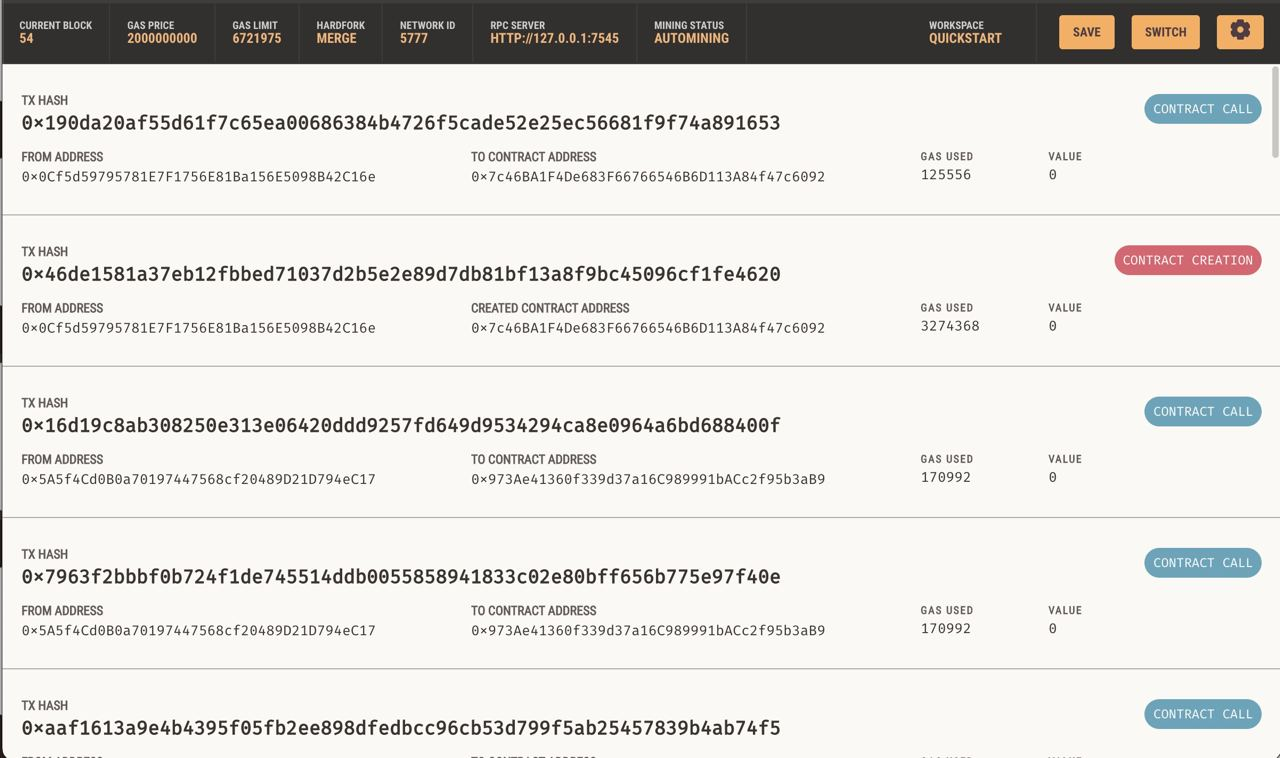
\includegraphics[scale=0.35]{gambar/ganache-uji-gas.jpg}

  % Ubah dengan keterangan gambar yang diinginkan
  \caption{Transaksi blockchain di Ganache}
  \label{fig:ganachegastest}
\end{figure}

Tujuan dari pengujian ini adalah untuk mengetahui berapa besar biaya gas yang dibutuhkan untuk menjalankan proses sistem pada Smart Contract yang sudah dibuat.
Proses dari pengujian ini sama seperti dengan Ganache network, hanya saja setiap proses sistem yang berjalan, lamanya waktu terkonfirmasi pada Metamask ditemukan variasi, yang mana
sangat berbeda dengan Ganache yang tidak memiliki jeda. Untuk method-method yang bersifat read only atau tidak payable dan tidak melakukan write operation tidak dilakukan
uji gas karena method-method tersebut tidak menggunakan gas untuk dieksekusi.

Dengan melakukan pengujian ini, pengembang dapat memperoleh pemahaman yang lebih baik tentang biaya gas yang terkait dengan menjalankan proses sistem pada Smart Contract. Informasi ini dapat digunakan untuk mengoptimalkan dan memperbaiki efisiensi penggunaan gas, serta memastikan bahwa Smart Contract berjalan secara optimal dengan biaya yang sesuai dan meminimalkan risiko transaksi yang tidak memadai.

\begin{enumerate}
  \item
        \textbf{Deployment Gas}

        Pengujian estimasi gas dimulai dari jaringan Ganache. Tabel dibawah ini menunjukan estimasi gas yang dibutuhkan untuk melakukan proses deploy Smart Contract pada Ganache

        \begin{longtable}{|c|c|c|}
          \caption{Hasil Pengujian Deploy Smart Contract}
          \label{tb:UjiDeploy}                                                                             \\
          \hline
          \rowcolor[HTML]{C0C0C0}
          \textbf{\emph{Blockchain Network}} & \textbf{\emph{Gas Used}} & \textbf{\emph{Gas Price (Gwei)}} \\
          \hline
          Ganache                            & 3274368                  & 2.772126468                      \\
          Goerli                             & 3275354                  & 2.500000024                      \\
          Sepolia                            & 3275354                  & 2.500000012                      \\
          \hline
        \end{longtable}

        \begin{longtable}{|c|c|c|}
          \caption{Hasil Pengujian Deploy Smart Contract di \emph{Ganache}}
          \label{tb:UjiDeployGanache}                                                                \\
          \hline
          \rowcolor[HTML]{C0C0C0}
          \textbf{\emph{Percobaan ke}} & \textbf{\emph{Gas Used}} & \textbf{\emph{Gas Price (Gwei)}} \\
          \hline
          1                            & 3274368                  & 2.769504978                      \\
          2                            & 3274368                  & 2.77037599                       \\
          3                            & 3274368                  & 2.760107065                      \\
          4                            & 3274368                  & 2.760947704                      \\
          5                            & 3274368                  & 2.761791060                      \\
          6                            & 3274368                  & 2.762637142                      \\
          7                            & 3274368                  & 2.763485958                      \\
          8                            & 3274368                  & 2.764337517                      \\
          9                            & 3274368                  & 2.758433902                      \\
          10                           & 3274368                  & 2.759269134                      \\
          11                           & 3274368                  & 2.760107034                      \\
          12                           & 3274368                  & 2.77037569                       \\
          13                           & 3274368                  & 2.760108232                      \\
          14                           & 3274368                  & 2.761792302                      \\
          15                           & 3274368                  & 2.762633213                      \\
          \hline
        \end{longtable}

        Dari hasil tabel yang didapatkan diatas, didapati bahwa penggunaan gas cukup besar karena proses melakukan deploy memang membutuhkan resource yang tidak sedikit.
        Gas Used pada jaringan lokal Ganache juga lebih besar daripada di jaringan Goerli dan Sepolia. Pada tabel \ref{tb:UjiDeployGanache} juga dilakukan 10 kali percobaan
        yang mana hasilnya dapat disimpulkan bahwa gas price di jaringan lokal ganache lebih besar daripada Goerli dan Sepolia pada saat pengujian proses deployment smart contract.

  \item
        \textbf{Minting Gas}

        Pengujian efisiensi gas selanjutnya adalah pengujian saat melakukan minting token atau proses pembuatan NFT untuk menyimpan data URI.
        Proses ini sendiri memanggil method \texttt{mint} dan karena method ini bersifat write dan payable maka penggunaan gas nya pun akan lebih
        banyak dibandingkan method yang bersifat write. Pengujian ini akan dilakukan dengan jaringan lokal ganache dan juga jaringan Goerli dan Sepolia.
        Berikut ini adalah table hasil pengujian efisiensi gas untuk pemanggilan method mint pada smart contract.

        Pengujian efisiensi gas ini penting untuk memahami dan mengoptimalkan biaya yang dikeluarkan dalam proses pembuatan NFT dan penyimpanan data URI. Dengan mengetahui jumlah gas yang diperlukan, pengembang dapat mengambil langkah-langkah untuk meningkatkan efisiensi penggunaan gas dan meminimalkan biaya yang terkait dengan operasi-operasi tersebut pada smart contract.

        \begin{longtable}{|c|c|c|}
          \caption{Hasil Pengujian Gas Mint Smart Contract}
          \label{tb:UjiGasMint}                                                                            \\
          \hline
          \rowcolor[HTML]{C0C0C0}
          \textbf{\emph{Blockchain Network}} & \textbf{\emph{Gas Used}} & \textbf{\emph{Gas Price (Gwei)}} \\
          \hline
          Ganache                            & 170992                   & 2.526306790                      \\
          Goerli                             & 125580                   & 2.500000016                      \\
          Sepolia                            & 125568                   & 2.500000016                      \\
          \hline
        \end{longtable}

        \begin{longtable}{|c|c|c|}
          \caption{Hasil Pengujian Gas Mint di \emph{Ganache}}
          \label{tb:UjiGasMintGanache}                                                               \\
          \hline
          \rowcolor[HTML]{C0C0C0}
          \textbf{\emph{Percobaan ke}} & \textbf{\emph{Gas Used}} & \textbf{\emph{Gas Price (Gwei)}} \\
          \hline
          1                            & 170992                   & 2.526306790                      \\
          2                            & 170992                   & 2.529847969                      \\
          3                            & 170992                   & 2.533865829                      \\
          4                            & 170992                   & 2.538424537                      \\
          5                            & 170992                   & 2.543596897                      \\
          6                            & 170992                   & 2.549465512                      \\
          7                            & 170992                   & 2.556124107                      \\
          8                            & 170992                   & 2.764337517                      \\
          9                            & 170992                   & 2.758433902                      \\
          10                           & 170992                   & 2.759269134                      \\
          11                           & 170992                   & 2.526303233                      \\
          12                           & 170992                   & 2.529832132                      \\
          13                           & 170992                   & 2.533847239                      \\
          14                           & 170992                   & 2.538491925                      \\
          15                           & 170992                   & 2.543581052                      \\
          \hline
        \end{longtable}

        Dari tabel \ref{tb:UjiGasMintGanache} diatas dapat diketahui bahwasanya Gas Used pada method mint cukup besar untuk standard
        blockchain smart contract. Kemudian untuk pemakaian gas yang dilakukan di jaringan lokal ganache lebih besar daripada di jaringan Goerli
        maupun Sepolia. Hal ini memperkuat hasil dari uji deployment yang dilakukan sebelumnya karena disana juga pemakaian gas yang ada di jaringan lokal
        Ganache. Gas Price ditentukan oleh tingkat penggunaan jaringan blockchain tersebut, sehingga semakin banyak pengguna yang mengakses jaringan dari suatu
        blockchain maka akan semakin banyak juga gas price yang akan dikonsumsi.
\end{enumerate}


\subsection{Hasil Pembuatan Metadata dengan IPFS}
Pengujian untuk IPFS dilakukan dengan cara melakukan pencocokan metadata dengan OpenSea. Metadata yang distandarkan oleh OpenSea akan digunakan dalam sistem.

Dalam pengembangan aplikasi dengan Unreal Engine 5, penting untuk memastikan bahwa metadata yang diunggah ke IPFS sesuai dengan standar yang diterima oleh OpenSea. Hal ini penting karena kompatibilitas dengan OpenSea memungkinkan NFT yang dibuat dengan Unreal Engine 5 dapat diperdagangkan secara interoperabel di platform tersebut.

Dengan melakukan pencocokan metadata dengan standar OpenSea, pengembang dapat memastikan bahwa NFT yang dihasilkan oleh Unreal Engine 5 dapat diakses dan dikenali dengan benar oleh platform perdagangan yang kompatibel. Hal ini memungkinkan NFT tersebut untuk mendapatkan eksposur lebih luas dan meningkatkan likuiditas dan nilai jualnya.

Dalam proses pengujian, metadata yang dihasilkan oleh Unreal Engine 5 akan dibandingkan dengan standar metadata yang ditetapkan oleh OpenSea untuk memastikan kesesuaian dan konsistensi. Jika metadata sesuai dengan standar OpenSea, maka NFT yang dibuat dengan Unreal Engine 5 dapat diintegrasikan dengan lancar dalam ekosistem OpenSea dan mendapatkan manfaat dari fitur-fitur yang disediakan oleh platform tersebut.

Metadata yang dibuat di IPFS sudah dapat diakses melalui gatewaynya. Contohnya untuk nft-1.json adalah sebagai berikut.

\begin{figure}[H]
  \centering

  % Ubah dengan nama file gambar dan ukuran yang akan digunakan
  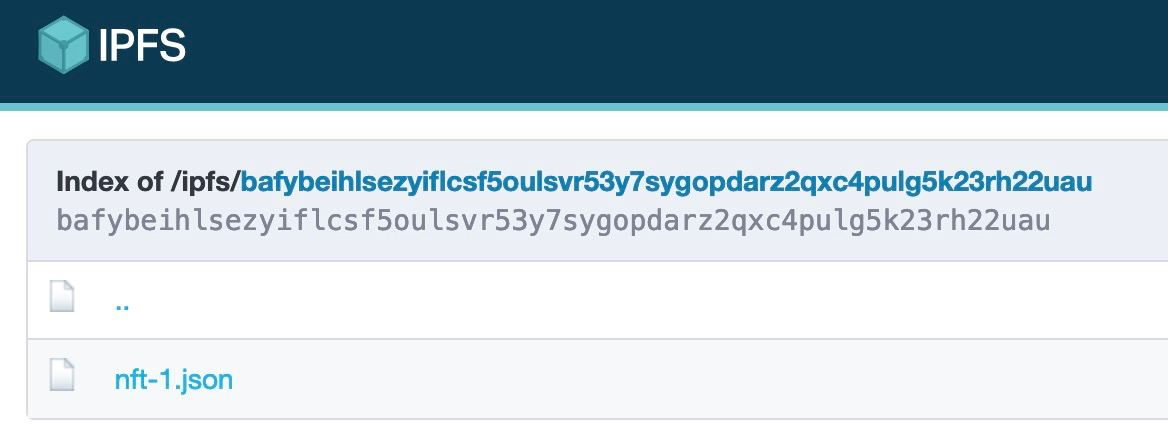
\includegraphics[scale=0.4]{gambar/nftjsonuploaded.jpg}

  % Ubah dengan keterangan gambar yang diinginkan
  \caption{Tampilan IPFS nft-1.json yang sudah diupload}
  \label{fig:ipfsjsonuploaded}
\end{figure}

Hasil dari pembacaan metadata pada OpenSea dengan jaringan testnet adalah dapat terbaca. Jika tidak digunakan standar metadata yang sudah menjadi konvensi
maka tidak akan terbaca oleh OpenSea apa yang sudah dituliskan pada metadata JSON yang diberikan pada jaringan blockchain OpenSea dalam bentuk mint file. Kemudian untuk
URI nya sendiri haruslah berupa URI valid, apabila tidak valid maka OpenSea juga tidak dapat membaca URI yang menyebabkan tidak dapat membaca metadata tersebut karena file metadata yang berupa JSON tersebut tersimpan
di dalam URI yang diberikan.

\begin{figure}[H]
  \centering

  % Ubah dengan nama file gambar dan ukuran yang akan digunakan
  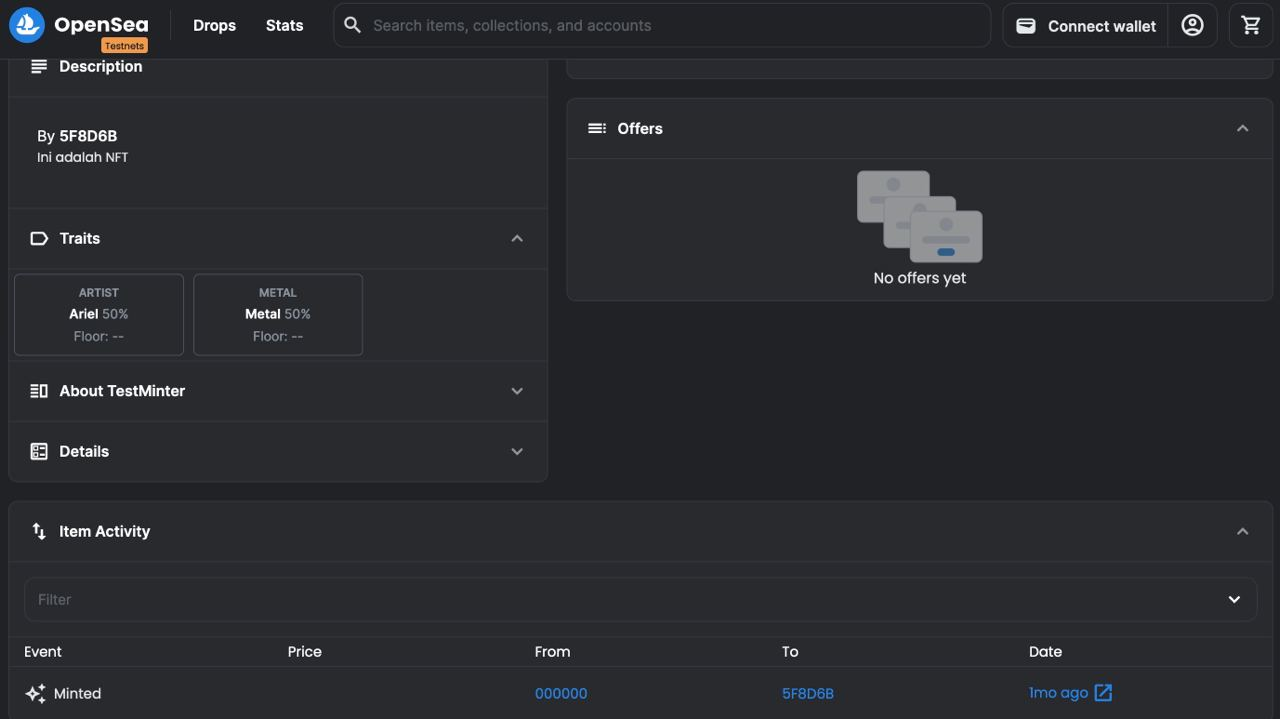
\includegraphics[scale=0.4]{gambar/opensea-uji.jpg}

  % Ubah dengan keterangan gambar yang diinginkan
  \caption{Tampilan OpenSea yang berhasil membaca metadata}
  \label{fig:openseatest}
\end{figure}

Penelitian ini menggunakan metadata yang sudah distandarkan oleh OpenSea, namun tidak ada pengecekan untuk formatnya itu sendiri sehingga apabila dimasukkan format yang salah maka integrasi dengan Unreal Engine 5 akan
gagal dan menyebabkan error yang detailnya akan dijelaskan pada pengujian-pengujian berikutnya.

Meskipun pengecekan format metadata tidak dilakukan dalam penelitian ini, hal tersebut merupakan langkah yang penting dalam pengembangan yang sebenarnya. Sebelum mengintegrasikan metadata dengan Unreal Engine 5, disarankan untuk memastikan bahwa metadata yang digunakan sesuai dengan format yang diharapkan untuk mencegah terjadinya kesalahan dan kegagalan integrasi yang dapat mempengaruhi fungsionalitas aplikasi.

\subsection{Hasil Mint NFT}
Pengujian ini berbeda dengan pengujian method \texttt{mint} yang ada pada pengujian-pengujian sebelumnya. Pada pengujian ini proses mint yang dimaksud adalah
proses dimana dilakukan deployment smart contract ke jaringan blockchain Goerli. Nantinya jaringan ini akan digunakan untuk integrasi dengan Unreal Engine 5.

Deployment smart contract ke jaringan Goerli dilakukan dengan akun yang sudah berisikan cukup GoerliETH karena proses deployment juga membutuhkan Ether.

\begin{longtable}{|c|c|}
  \caption{Hasil Pengujian Deploy ke Goerli berdasarkan Ether}
  \label{tb:UjiGoerliETH}                         \\
  \hline
  \rowcolor[HTML]{C0C0C0}
  \textbf{Jumlah GoerliETH} & \textbf{Keterangan} \\
  \hline
  12.5                      & Sukses              \\
  0                         & Gagal               \\
  0.001                     & Gagal               \\
  \hline
\end{longtable}

Dari tabel \ref{tb:UjiGoerliETH} dapat disimpulkan bahwa diperlukan jumlah GoerliETH yang memadai untuk dilakukannya proses deployment smart contract.
Minimum GoerliETH  untuk dilakukan deployment adalah 0.01 untuk batas amannya. Namun perlu diperhatikan juga bahwa proses mint URI tetap membutuhkan GoerliETH juga
sehingga perlu disiapkan GoerliETH yang cukup. GoerliETH didapat secara mining pada faucet-faucet yang tersedia di internet.

Hasil dari mint nft sudah dapat digunakan untuk integrasi Unreal Engine 5. ABI dapat dilihat pada compiler Remix IDE.
\begin{figure}[H]
  \centering

  % Ubah dengan nama file gambar dan ukuran yang akan digunakan
  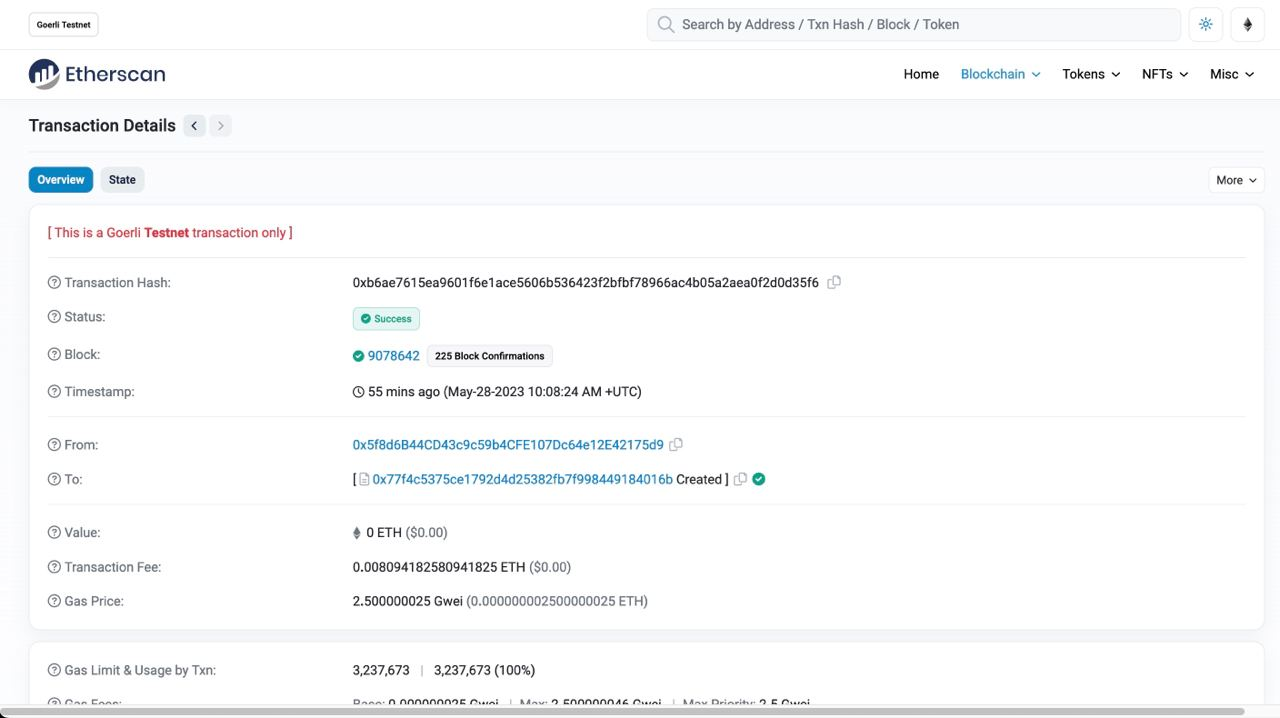
\includegraphics[scale=0.35]{gambar/etherscan-deploy.jpg}

  % Ubah dengan keterangan gambar yang diinginkan
  \caption{Etherscan dari hasil transaction mint NFT}
  \label{fig:etherscandeploy}
\end{figure}

ABI yang dapat dilihat di etherscan dapat digunakan pada integrasi Unreal Engine 5. Hal ini dilakukan agar
Unreal Engine 5 dapat membaca method-method apa saja yang terdapat pada smart contract. Kemudian diperlukan juga
alamat contract yang sudah dideploy agar Unreal Engine 5 yang sudah mengetahui spesifikasi smart contract dapat melakukan read data
yang sudah tersimpan dengan pemanggilan mint sebelumnnya.

Dengan menggunakan ABI yang dapat dilihat di etherscan, Unreal Engine 5 dapat melakukan integrasi dengan smart contract yang sudah dideploy. ABI (Application Binary Interface) adalah deskripsi formal dari method dan variabel yang ada dalam smart contract. Dengan mengetahui ABI dari smart contract, Unreal Engine 5 dapat memahami dan berinteraksi dengan method-method yang terdapat dalam smart contract tersebut.

Selain itu, untuk dapat membaca data yang sudah tersimpan di smart contract, Unreal Engine 5 juga memerlukan alamat contract yang sudah dideploy di blockchain. Dengan mengetahui alamat contract, Unreal Engine 5 dapat melakukan pemanggilan ke smart contract tersebut dan mengakses data yang sudah tersimpan di dalamnya.

Proses ini memungkinkan Unreal Engine 5 untuk mengintegrasikan dan menggunakan data yang ada di dalam smart contract dalam pengembangan dan simulasi metaverse. Dengan memanggil method-method yang terdapat dalam smart contract, Unreal Engine 5 dapat membaca, memperbarui, atau menggunakan data yang ada di dalamnya sesuai dengan kebutuhan pengembangan aplikasi atau simulasi metaverse yang sedang dilakukan.

Dengan adanya integrasi ini, Unreal Engine 5 dapat memanfaatkan potensi penuh dari smart contract dalam membangun pengalaman metaverse yang lebih dinamis, interaktif, dan terkoneksi dengan teknologi blockchain.

\subsection{Hasil Pembuatan Project Pada Unreal Engine 5}
Project unreal engine 5 yang sudah dibuat dapat memberikan environment visual yang dapat melakukan visualisasi audio maupun game.
Digunakan juga beberapa plugin yang dapat membantu proses integrasi.

\begin{figure}[H]
  \centering

  % Ubah dengan nama file gambar dan ukuran yang akan digunakan
  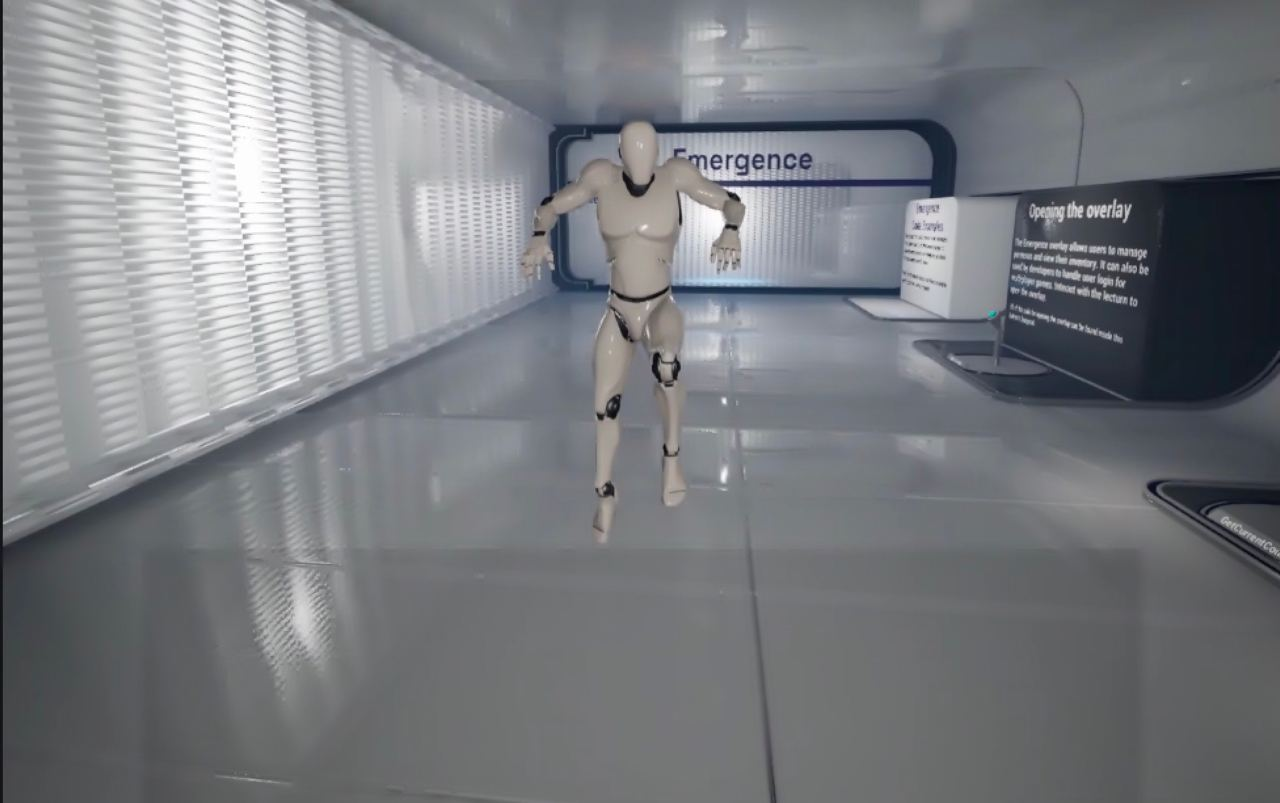
\includegraphics[scale=0.35]{gambar/ue5project.jpg}

  % Ubah dengan keterangan gambar yang diinginkan
  \caption{Tampilan project unreal engine 5}
  \label{fig:ue5project}
\end{figure}

Avatar yang disediakan oleh Unreal Engine 5 dapat digunakan untuk melakukan simulasi Metaverse.
Pada pengujian dilakukan operasi pergerakan avatar dan melakukan penginstallan plugin-plugin web3 yang dapat membantu proses integrasi.
Selain itu, Unreal Engine 5 juga menyediakan avatar yang dapat digunakan untuk melakukan simulasi di dalam metaverse. Avatar tersebut memungkinkan pengguna untuk menciptakan representasi digital dari diri mereka sendiri atau karakter yang mereka pilih, dan berinteraksi dengan lingkungan dan pengguna lain di dalam metaverse.

Selama pengujian, dilakukan operasi pergerakan avatar untuk menguji kemampuan navigasi dan interaksi di dalam metaverse. Selain itu, pengujian juga melibatkan penginstalan plugin-plugin web3 yang dirancang khusus untuk Unreal Engine 5. Plugin-plugin ini membantu proses integrasi dengan teknologi Web3, seperti blockchain dan smart contract, sehingga memungkinkan pengguna untuk terlibat dalam transaksi dan aktivitas berbasis kripto di dalam metaverse.

Dengan adanya fitur avatar dan integrasi dengan plugin-plugin web3, Unreal Engine 5 memberikan kesempatan bagi pengembang dan pengguna untuk merasakan pengalaman yang lebih mendalam dan interaktif di dalam metaverse. Pengguna dapat menjelajahi lingkungan yang dirancang dengan detail, berinteraksi dengan avatar lain, melakukan transaksi menggunakan kriptocurrency, dan terlibat dalam aktivitas-aktivitas kreatif dan sosial yang unik di dalam metaverse.

Dalam keseluruhan, Unreal Engine 5 memainkan peran penting dalam memfasilitasi simulasi metaverse dengan menyediakan fitur avatar yang dapat digunakan untuk mewakili pengguna dan integrasi dengan plugin-plugin web3. Hal ini memungkinkan pengembang dan pengguna untuk terlibat dalam pengalaman metaverse yang lebih imersif, dinamis, dan terkoneksi dengan teknologi blockchain.

\subsection{Hasil Integrasi Kontrak dengan Unreal Engine 5}

Setelah diintegrasikan dengan blueprint maka di lingkungan virtual unreal engine 5 sudah dapat memutar audio yang didapatkan dari NFT.
Blueprint yang digunakan adalah sebagai berikut.

\begin{figure}[H]
  \centering

  % Ubah dengan nama file gambar dan ukuran yang akan digunakan
  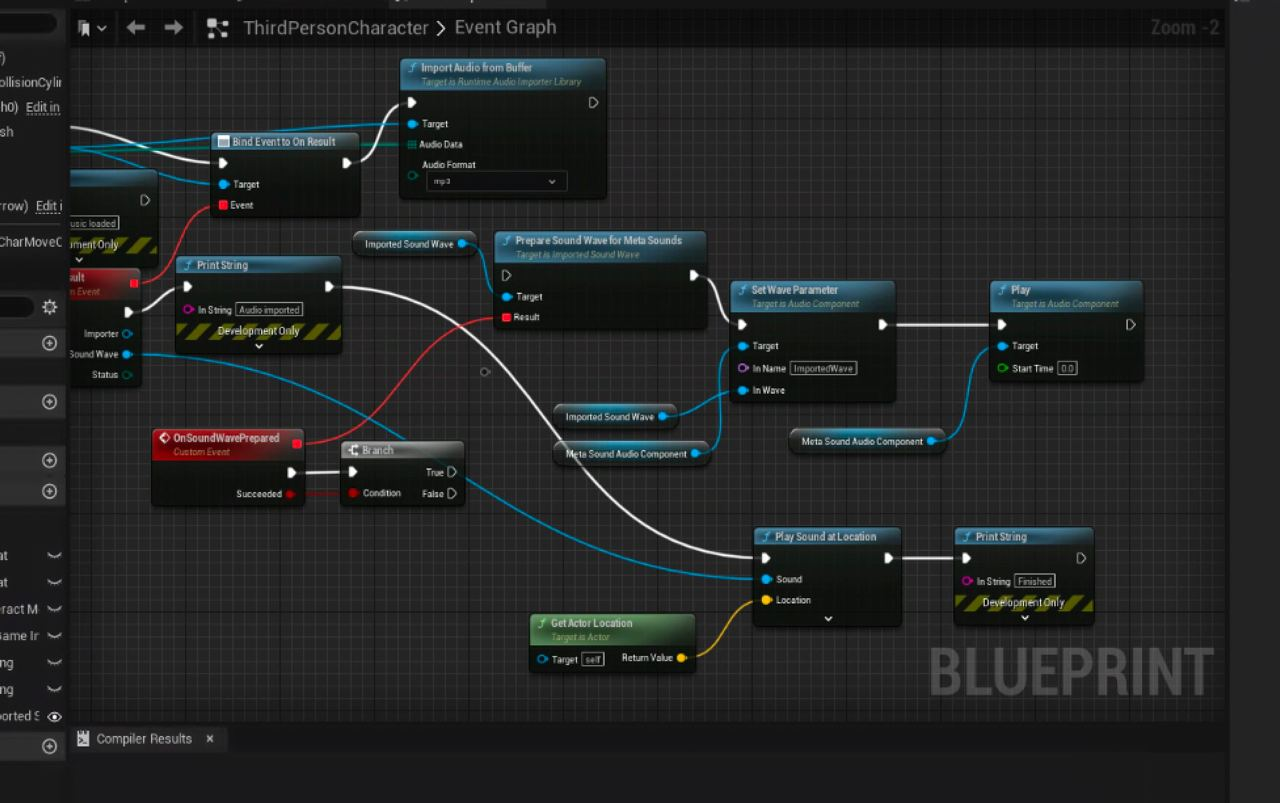
\includegraphics[scale=0.35]{gambar/blueprintfinal.jpg}

  % Ubah dengan keterangan gambar yang diinginkan
  \caption{Tampilan blueprint final}
  \label{fig:blueprintfinal}
\end{figure}

Pengujian yang akan dilakukan adalah berhasil tidaknya integrasi dengan cara
melakukan pemutaran audio dengan menggunakan metadata yang sudah di mint pada proses sebelumnya.
Akan dilakukan beragam cara yakni menggunakan ABI yang tidak valid dan juga sebaliknya.

\begin{figure}[H]
  \centering

  % Ubah dengan nama file gambar dan ukuran yang akan digunakan
  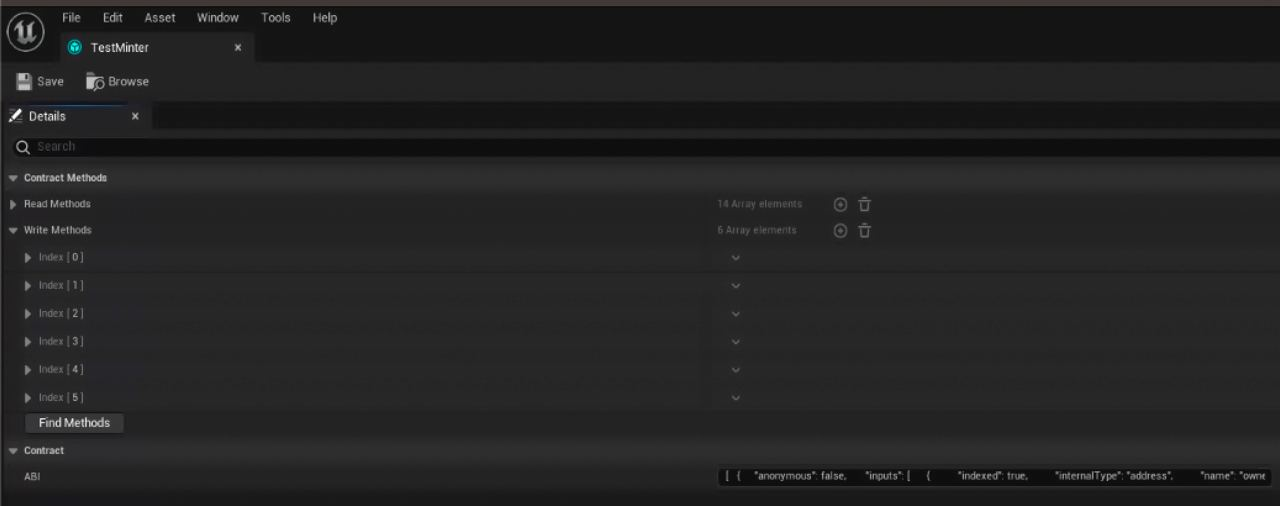
\includegraphics[scale=0.35]{gambar/contract-abi.jpg}

  % Ubah dengan keterangan gambar yang diinginkan
  \caption{Tampilan contract ABI di Unreal Engine 5}
  \label{fig:contractabiue5}
\end{figure}

\begin{longtable}{|c|c|}
  \caption{Hasil Pengujian ABI Smart Contract di UE5}
  \label{tb:UjiIntegrasiUE5ABI}               \\
  \hline
  \rowcolor[HTML]{C0C0C0}
  \textbf{Contract ABI} & \textbf{Keterangan} \\
  \hline
  Valid                 & Sukses              \\
  Invalid               & Gagal               \\
  \hline
\end{longtable}

Dari tabel di atas, dapat disimpulkan bahwa keberhasilan integrasi tergantung pada validitas Contract ABI. Jika Contract ABI tidak valid, proses integrasi tidak dapat dilakukan karena langkah pertama yang harus dilakukan adalah
menyediakan Contract ABI yang benar. Contract ABI digunakan sebagai deskripsi antarmuka dari smart contract yang akan diintegrasikan, dan kesalahan dalam Contract ABI dapat menghambat atau menyebabkan kegagalan integrasi dengan Unreal Engine 5. Oleh karena itu, penting untuk memastikan keakuratan dan kevalidan Contract ABI sebelum melanjutkan proses integrasi.

Selanjutnya adalah pengujian proses pemanggilan smart contract di Unreal Engine 5. Pada proses ini
blueprint yang digunakan akan memanggil method-method read yang ada pada smart contract yang sudah dibaca dalam tahapan pemberian Contract ABI sebelumnya seperti \texttt{tokenURI}, \texttt{getAllTokens}, dan \texttt{getAllTokensURI}. Dengan memanggil method tersebut diharapkan dapat dimuat metadata JSON yang sudah di \texttt{mint}
pada tahapan sebelumnya.

\begin{longtable}{|c|c|c|c|c|}
  \caption{Hasil Pengujian Pemanggilan method menggunakan Blueprint}
  \label{tb:UjiPemanggilanMethod}                                                               \\
  \hline
  \rowcolor[HTML]{C0C0C0}
  \textbf{Method} & \textbf{Alamat Contract} & \textbf{Sesuai Dengan ABI} & \textbf{Keterangan} \\
  \hline
  tokenURI        & Valid                    & true                       & Sukses              \\
  tokenURI        & Invalid                  & true                       & Gagal               \\
  tokenURI        & Valid                    & false                      & Gagal               \\
  tokenURI        & Invalid                  & false                      & Gagal               \\
  getAllTokens    & Valid                    & true                       & Sukses              \\
  getAllTokens    & Invalid                  & true                       & Gagal               \\
  getAllTokens    & Valid                    & false                      & Gagal               \\
  getAllTokens    & Invalid                  & false                      & Gagal               \\
  getAllTokensURI & Valid                    & true                       & Sukses              \\
  getAllTokensURI & Invalid                  & true                       & Gagal               \\
  getAllTokensURI & Valid                    & false                      & Gagal               \\
  getAllTokensURI & Invalid                  & false                      & Gagal               \\
  \hline
\end{longtable}

Dari tabel diatas dapat diketahui bahwa apabila alamat contract yang diberikan tidak valid atau tidak cocok maka
akan terjadi error sehingga menyebabkan proses integrasi gagal.
Jika alamat contract valid dan cocok dengan ABI dan contract juga valid maka pembacaan method akan mengembalikan nilai yang benar.
Blueprint Unreal Engine 5 akan meneruskan balikan dari pemanggilan method smart contract ini untuk diproses pada blueprint-blueprint selanjutnya.

\begin{figure}[H]
  \centering

  % Ubah dengan nama file gambar dan ukuran yang akan digunakan
  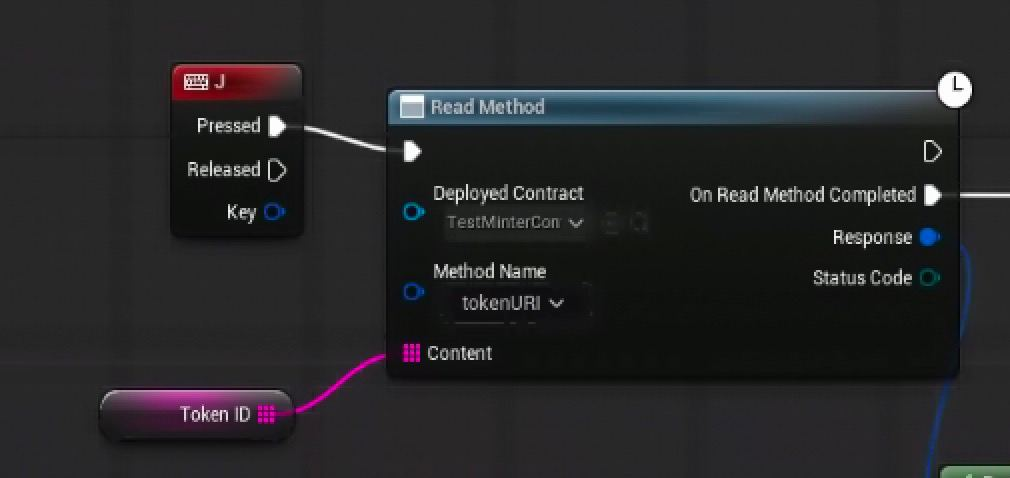
\includegraphics[scale=0.35]{gambar/blueprint-tokenuri.jpg}

  % Ubah dengan keterangan gambar yang diinginkan
  \caption{Tampilan blueprint untuk pemanggilan method \texttt{tokenURI}}
  \label{fig:blueprinttokenuri}
\end{figure}

Blueprint-blueprint lainnya dalam Unreal Engine 5 dapat menggunakan nilai yang dikembalikan
dari pemanggilan method smart contract untuk melanjutkan proses selanjutnya. Dengan demikian, integrasi yang
berhasil antara Unreal Engine 5 dan smart contract memungkinkan penggunaan data blockchain dalam
pengembangan aplikasi atau permainan. Hal ini membuka peluang untuk menciptakan pengalaman unik yang berbasis pada transaksi
dan kepemilikan aset digital, seperti NFT. Blueprint-blueprint selanjutnya dapat menggunakan data dari smart contract untuk mengatur logika permainan,
mengatur kepemilikan aset, atau bahkan memungkinkan interaksi dengan NFT yang dimiliki oleh pemain. Dengan adanya integrasi ini,
Unreal Engine 5 dapat menjadi platform yang kuat untuk membangun pengalaman Metaverse yang terhubung dengan blockchain.

\begin{figure}[H]
  \centering

  % Ubah dengan nama file gambar dan ukuran yang akan digunakan
  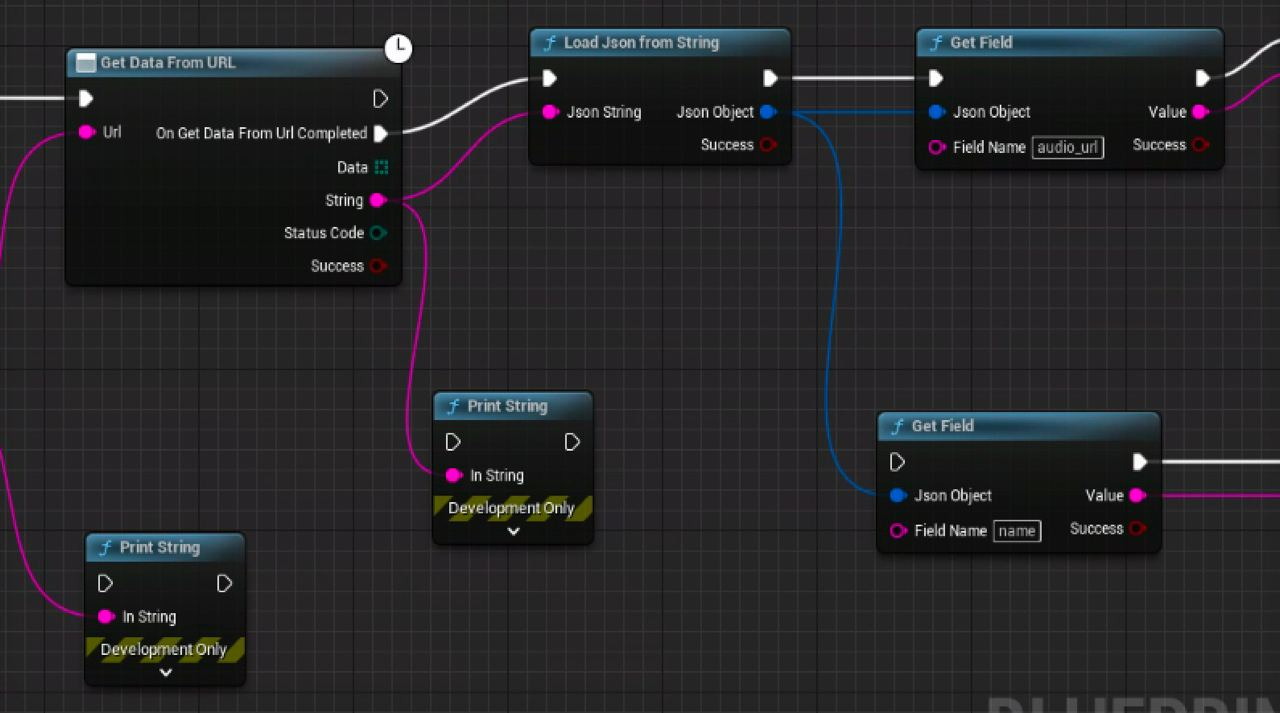
\includegraphics[scale=0.35]{gambar/blueprint-load-metadata.jpg}

  % Ubah dengan keterangan gambar yang diinginkan
  \caption{Tampilan blueprint untuk load metadata}
  \label{fig:blueprintloadmetadata}
\end{figure}

Selanjutnya adalah pengujian integrasi dengan pembacaan format metadata. Format metadata audio yang sudah dibaca pada proses sebelumnya akan diteruskan ke blueprint berikutnya.
Berikut ini adalah tabel hasil pengujian proses memuat metadata.

\begin{longtable}{|c|c|c|}
  \caption{Hasil Pengujian Load Metadata Audio di UE5}
  \label{tb:UjiIntegrasiPengujianLoadMetadataAudio}                                    \\
  \hline
  \rowcolor[HTML]{C0C0C0}
  \textbf{JSON Key di Metadata} & \textbf{JSON Key di Blueprint} & \textbf{Keterangan} \\
  \hline
  audio\_url                    & audio\_url                     & Sukses              \\
  music\_url                    & audio\_url                     & Gagal               \\
  music\_url                    & music\_url                     & Sukses              \\
  audio\_url                    & music\_url                     & Gagal              \\
  \hline
\end{longtable}

Dari tabel diatas dapat diketahui bahwa jika format metadata yang diberikan tidak valid maka akan terjadi error karena file JSON yang dibaca
akan diambil key \texttt{audio\_url}-nya, sehingga jika tidak terdapat key \texttt{audio\_url} maka haruslah terjadi error. Ini adalah hasil yang dikehendaki.

Ketika keseluruhan data yang diberikan valid maka dapat dilanjutkan ke proses pengujian berikutnya yaitu proses pemutaran audio secara \emph{real time}.
Biasanya file audio asset pada game akan dimuat secara lokal, namun tidak dengan sistem ini dimana file yang akan diputar adalah file yang berasal dari internet.

File ini dimuat dengan membaca smart contract dan membaca audio url di dalam metadata yang ada di NFT pada smart contract. Untuk eksperimen berikut akan dilakukan
dengan cara mencoba beberapa file audio yang akan di putar oleh runtime audio importer.

\begin{longtable}{|c|c|c|}
  \caption{Hasil Pengujian Pemutaran Audio di Unreal Engine 5}
  \label{tb:UjiIntegrasiPemutaranAudio}                       \\
  \hline
  \rowcolor[HTML]{C0C0C0}
  \textbf{Audio format} & \textbf{Size} & \textbf{Keterangan} \\
  \hline
  mp3                   & 5mb           & Sukses              \\
  mp3                   & 10mb          & Sukses              \\
  mp3                   & 1000mb        & Gagal               \\
  wav                   & 300kb         & Sukses              \\
  wav                   & 5mb           & Sukses              \\
  wav                   & 10mb          & Sukses              \\
  flac                  & 5mb           & Sukses              \\
  flac                  & 10mb          & Sukses              \\
  ogg                   & 5mb           & Gagal               \\
  ogg                   & 10mb          & Gagal               \\
  \hline
\end{longtable}

Dari hasil pengujian diketahui bahwa format data yang disupport hanyalah mp3 saja, sementara untuk ukuran file juga berpengaruh.
Semakin besar ukuran file maka waktu tunggu juga semakin lama. Akan tetapi karena file audio dimuat dalam memori jika ukuran file terlalu besar maka
akan terjadi crash.

\section{Evaluasi Pengujian}
Berdasarkan pengujian yang telah dilakukan, pengujian sistem Sharing Data berbasis blockchain di metaverse dapat berjalan sebagaimana mestinya.
Method \emph{mint} pada \emph{smart contract} hanya akan gagal apabila string yang diberikan kosong. Method \emph{getAllTokens} akan mengembalikan array sepanjang banyaknya jumlah
pemanggilan \emph{mint}. Lalu untuk method \emph{getAllTokensURI} akan mengembalikan array yang berisi URI yang sudah pernah di-\emph{mint} sebelumnya.

Kemudian untuk pengujian \emph{method} \texttt{tokenURI} diketahui bahwa \emph{method} ini akan mengembalikan URI yang sesuai dengan urutan pemanggilan \texttt{mint}.
URI tersebut disimpan dalam bentuk array sehingga apabila diberikan parameter bilangan yang tidak di dalam \emph{range} \emph{array} tersebut maka akan terjadi \emph{error}.
Kemudian terdapat juga pengujian gas dari proses \emph{deploy smart contract} dan juga pemanggilan \emph{mint}. Diperoleh bahwa pemakaian gas tertinggi didapatkan ketika dilakukan proses
\emph{deployment}. Lalu untuk \emph{Gas Used} yang paling banyak digunakan diantara \emph{test net} adalah Goerli. Lalu untuk pemanggilan \emph{smart contract method} dengan \emph{UE5 blueprint} didapati bahwa
hanya akan sukses apabila ABI dan alamat \emph{contract} yang diberikan valid. Lalu untuk jenis file yang didukung adalah file dengan format mp3, wav, dan flac. Sementara ogg belum mendapat \emph{support}.
Untuk ukuran file juga mempengaruhi delay daripada pemutaran audio ini, dengan file mp3 pada pengujian yang berukuran 1000mb maka akan terjadi gagal.

